% BEGIN LICENSE BLOCK
% Version: CMPL 1.1
%
% The contents of this file are subject to the Cisco-style Mozilla Public
% License Version 1.1 (the "License"); you may not use this file except
% in compliance with the License.  You may obtain a copy of the License
% at www.eclipse-clp.org/license.
% 
% Software distributed under the License is distributed on an "AS IS"
% basis, WITHOUT WARRANTY OF ANY KIND, either express or implied.  See
% the License for the specific language governing rights and limitations
% under the License. 
% 
% The Original Code is  The ECLiPSe Constraint Logic Programming System. 
% The Initial Developer of the Original Code is  Cisco Systems, Inc. 
% Portions created by the Initial Developer are
% Copyright (C) 2006 Cisco Systems, Inc.  All Rights Reserved.
% 
% Contributor(s): 
% 
% END LICENSE BLOCK

%----------------------------------------------------------------------
\chapter{Program Analysis}
\label{sec:program-analysis}
\index{program analysis|(}
%HEVEA\cutdef[1]{section}
%----------------------------------------------------------------------

This chapter describes some of the tools provided by \eclipse{} to
analyse the runtime behaviour of a program.
\index{performance}\index{optimisation}
%----------------------------------------------------------------------
\section{What tools are available?}
%----------------------------------------------------------------------

\eclipse{} provides a number of different tools to help the programmer
understand their how their program behaves at runtime.

\quickrefstatic{Available Program Analysis tools}{
\begin{small}
\begin{description}
\item[Debugger] Provides a low level view of program
activity. \See{See chapter~\ref{chapdebug} and the \emph{Debugging}
section in the user manual for a comprehensive look at debugging
\eclipse{} programs}
\item[Profiler] Samples the running program at regular intervals to
give a statistical summary of where the execution time is spent.
\item[Port Profiler] Collects statistics about program execution in terms
of the box model of execution. See library(port_profiler) or use the
\emph{Port Profile} option from the tkeclipse \emph{Run} menu.
\item[Coverage] Records the number of times various parts of the
program are executed.
\item[Visualisation framework] \See{See the \emph{Visualisation Tools Manual} for more information}
\end{description}
\end{small}
}

This section focuses on two complementary tools
\begin{enumerate}
\item The \emph{profiler}
\item The \emph{coverage} library
\end{enumerate}

%----------------------------------------------------------------------
\section{Profiler}
%----------------------------------------------------------------------

\index{profiling} The profiling tool helps to find \emph{hot spots} in
a program that are worth optimising. It can be used any time with any
compiled Prolog code, it is not necessary to use a special compilation
mode or set any flags.  Note however that it is not available on
Windows\index{windows}.  When
\begin{quote}\begin{verbatim}
?- profile(Goal).
\end{verbatim}\end{quote}
\index{profile/1} is called, the profiler executes the \emph{Goal} in
the profiling mode, which means that every 100th of a second the
execution is interrupted and the profiler records the currently
executing procedure.

Consider the following \textbf{n-queens} code.
\begin{code}
queen(Data, Out) :-
        qperm(Data, Out),
        safe(Out).

qperm([], []).
qperm([X|Y], [U|V]) :-
        qdelete(U, X, Y, Z),
        qperm(Z, V).

qdelete(A, A, L, L).
qdelete(X, A, [H|T], [A|R]) :-
        qdelete(X, H, T, R).

safe([]).
safe([N|L]) :-
        nodiag(L, N, 1),
        safe(L).

nodiag([], _, _).
nodiag([N|L], B, D) :-
        D =\verb+\+= N - B,
        D =\verb+\+= B - N,
        D1 is D + 1,
        nodiag(L, B, D1).
\end{code}

Issuing the following query will result in the profiler recording the
currently executing goal 100 times a second.

\begin{quote}\begin{verbatim}
?- profile(queen([1,2,3,4,5,6,7,8,9],Out)).
goal succeeded

                PROFILING STATISTICS
                --------------------

Goal:             queen([1, 2, 3, 4, 5, 6, 7, 8, 9], Out)
Total user time:  0.03s

Predicate             Module        %Time   Time   %Cum
--------------------------------------------------------
qdelete           /4  eclipse       50.0%   0.01s  50.0%
nodiag            /3  eclipse       50.0%   0.01s 100.0%

Out = [1, 3, 6, 8, 2, 4, 9, 7, 5]
Yes (0.14s cpu)
\end{verbatim}\end{quote}

From the above result we can see how the profiler output contains four
important areas of information:
\begin{enumerate}
\item The first line of output indicates whether the specified goal
\textbf{succeeded}, \textbf{failed} or \textbf{aborted}.  The
\verb+profile/1+ predicate itself always succeeds.
\item The line beginning \verb+Goal:+ shows the goal which was
profiled.
\item The next line shows the time spent executing the goal.
\item Finally the predicates which were being executed when the
profiler sampled, ranked in decreasing sample count order are shown.
\end{enumerate}

The problem with the results displayed above is that the sampling
frequency is too low when compared to the total user time spent
executing the goal.  In fact in the above example the profiler was
only able to take two samples before the goal terminated.

The frequency at which the profiler samples is fixed, so in order to
obtain more representative results one should have an auxiliary
predicate which calls the goal a number of times, and compile and
profile a call to this auxiliary predicate. eg.

\begin{code}
queen_100 :-
  (for(_,1,100,1) do queen([1,2,3,4,5,6,7,8,9],_Out)).
\end{code}

Note that, when compiled, the above \verb+do/2+ loop would be
efficiently implemented and not cause overhead that would distort the
measurement.  \See{See section \ref{sec:loops} for more information on
logical loops}

\begin{quote}\begin{verbatim}
?- profile(queen_100).
goal succeeded

                PROFILING STATISTICS
                --------------------

Goal:             queen_100
Total user time:  3.19s

Predicate             Module        %Time   Time   %Cum
--------------------------------------------------------
nodiag            /3  eclipse       52.2%   1.67s  52.2%
qdelete           /4  eclipse       27.4%   0.87s  79.6%
qperm             /2  eclipse       17.0%   0.54s  96.5%
safe              /1  eclipse        2.8%   0.09s  99.4%
queen             /2  eclipse        0.6%   0.02s 100.0%

Yes (3.33s cpu)
\end{verbatim}\end{quote}

In the above example, the profiler takes over three hundred samples
resulting in a more accurate view of where the time is being spent in
the program.  In this instance we can see that more than half of the
time is spent in the \verb+nodiag/3+ predicate, making it an ideal
candidate for optimisation.  This is left as an exercise for the
reader.


%----------------------------------------------------------------------
\section{Line coverage}
%----------------------------------------------------------------------
\index{library!coverage}
\index{coverage}
\index{line coverage}
The line coverage library provides a means to ascertain exactly how
many times individual clauses are called during the evaluation of a
query.

\index{coverage counters}
The library works by placing \emph{coverage counters} at strategic
points throughout the code being analysed.  These counters are
incremented each time the evaluation of a query passes them.  There
are three locations in which coverage counters can be inserted.
\quickrefstatic{Locations where coverage counters can be placed}{
\begin{enumerate}
\item At the beginning of a code block.
\item Between predicate calls within a code block.
\item At the end of a code block.
\end{enumerate}
}
A code block is defined to be a conjunction of predicate calls. ie. a
sequence of goals separated by commas.

As previously mentioned, by default, code coverage counters are
inserted before and after every subgoal in the code. For instance, in
the clause
\begin{code}
p :- q, r, s.
\end{code}
four counters would be inserted: before the call to \verb+q+, between
\verb+q+ and \verb+r+, between \verb+r+ and \verb+s+, and after
\verb+s+:
\begin{quote}\begin{verbatim}
p :- point(1), q, point(2), r, point(3), s, point(4).
\end{verbatim}\end{quote}


This is the most precise form provided. The counter values do not only
show whether all code points were reached but also whether subgoals
failed or aborted (in which case the counter before a subgoal will
have a higher value than the counter after it). For example, the
result of running the above code is:
\begin{quote}\begin{alltt}
p :- \HighGreen{43 } q, \HighGreen{25 } r, \HighGreen{25 } s \HighRed{0 } .
\end{alltt}\end{quote}

which indicates that \verb+q+ was called 43 times, but succeeded only
25 times, \verb+r+ was called 25 times and succeeded always, and
\verb+s+ was called 25 times and never succeeded. Coverage counts of
zero are displayed in red (the final box) because they indicate
unreached code.  The format of the display is explained in the next
section.

%----------------------------------------------------------------------
\subsection{Compilation}
%----------------------------------------------------------------------
\index{ccompile/1}
\index{ccompile!coverage}
In order to add the coverage counters to code, it must be compiled with
the \bipref{ccompile/1}{../bips/lib/coverage/ccompile-1.html}
predicate which can be found in the
\bipref{coverage}{../bips/lib/coverage/index.html} library.

The predicate \verb+ccompile/1+ (note the initial `c' stands for
coverage) can be used in place of the normal \verb+compile/1+
predicate to compile a file with coverage counters.

Here we see the results of compiling the \textbf{n-queens} example
given in the previous section.
\begin{quote}\begin{verbatim}
?- coverage:ccompile(queens).
coverage: inserted 22 coverage counters into module eclipse
foo.ecl    compiled traceable 5744 bytes in 0.00 seconds

Yes (0.00s cpu)
\end{verbatim}\end{quote}

Once compiled, predicates can be called as usual and will (by default)
have no visible side effects.  Internally however, the counters will
be incremented as the execution progresses.  To see this in action,
consider issuing the following query having compiled the previously
defined code using \verb+ccompile/1+.
\begin{quote}\begin{alltt}
?- queens([1,2,3,4,5,6,7,8,9], Out).
\end{alltt}\end{quote}

The default behaviour of the \verb+ccompile/1+ predicate is to place
coverage counters as explained above, however such a level of detail
may be unnecessary.  If one is interested in reachability analysis the
two argument predicate \verb+ccompile/2+ \index{ccompile/2}
\index{ccompile!coverage} can take a list of \verb+name:value+ pairs
which can be used to control the exact manner in which coverage
counters are inserted.\See{See
\bipref{ccompile/2}{../bips/lib/coverage/ccompile-2.html} for a
full list of the available flags.}  In particular by specifying the
option \verb+blocks_only:on+, counters will only be inserted at the
beginning and end of code blocks. Reusing the above example this would
result in counters at point(1) and point(4).

\begin{quote}\begin{alltt}
p :- \HighGreen{43 } q,  r,  s \HighRed{0 } .
\end{alltt}\end{quote}

This can be useful in tracking down unexpected failures by looking for
exit counters which differ from entry counters, for example.


%----------------------------------------------------------------------
\subsection{Results}
%----------------------------------------------------------------------

\index{result/1} \index{result!coverage} To generate an html file
containing the coverage counter results issue the following query.
\begin{quote}\begin{verbatim}
?- coverage:result(queens).
\end{verbatim}\end{quote}
This will create the result file \texttt{coverage/queens.html} which
can be viewed using any browser.  It contains a pretty-printed form of
the source, annotated with the values of the code coverage counters as
described above. An example is shown in figure \ref{fig:queens}.

\begin{figure}
\begin{center}
\resizebox{0.5\textwidth}{!}{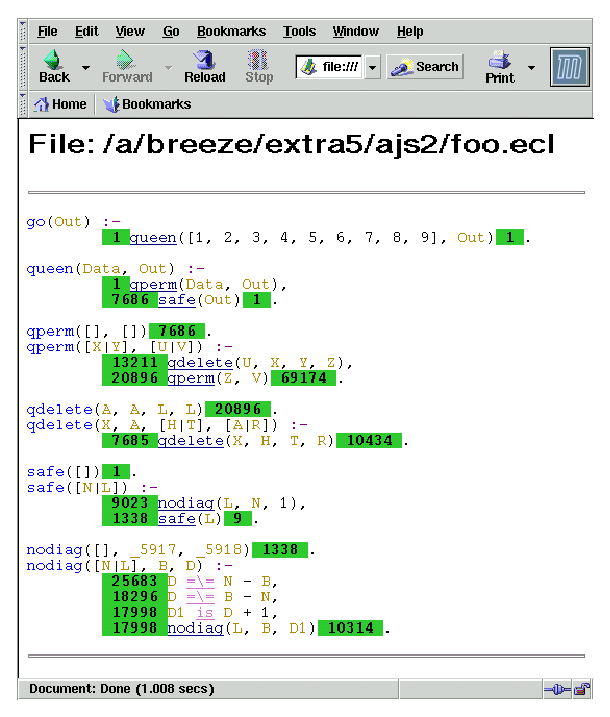
\includegraphics{coverage.eps}}
\end{center}
\caption{Results of running queens([1,2,3,4,5,6,7,8,9],_)}
\label{fig:queens}
\end{figure}

\index{result/0} \index{result!coverage} For extra convenience the
predicate \verb+result/0+ is provided which will create results for
all files which have been compiled with coverage counters.

\quickref{Result generating commands}{
\begin{description}
\item[\bipref{result/0}{../bips/lib/coverage/result-0.html}] Creates
results for all files which have been compiled with coverage counters.
\item[\bipref{result/1}{../bips/lib/coverage/result-1.html}] This
predicate takes a single argument which is the name of the file to
print the coverage counters for.
\item[\bipref{result/2}{../bips/lib/coverage/result-2.html}]
\index{result/2} The result predicate has a two argument form, the
second argument defining a number of flags which control (amongst
other things)
\begin{itemize}
\item The directory in which to create the results file. Default:
\texttt{coverage}.
\item The format of the results file (html or text). Default:
\texttt{html}.
\end{itemize}
\end{description}
\See{See \bipref{coverage}{../bips/lib/coverage/index.html} library
and \bipref{pretty_printer}{../bips/lib/pretty_printer/index.html}
library for more details}
}

\index{reset_counters/0} \index{reset_counters!coverage} Having
generated and viewed results for one run, the coverage counters can be
reset by calling
\begin{quote}\begin{verbatim}
?- coverage:reset_counters.

Yes (0.00s cpu)
\end{verbatim}\end{quote}

\index{program analysis|)}
%HEVEA\cutend
